\cleardoublepage
\chapter{Verifikation}
\label{ch:Verifikation}

Nach der Implementierung des Konzepts wird in diesem Kapitel überprüft, inwieweit das umgesetzte System die zu Beginn gestellten Anforderungen erfüllt. Dieser Schritt ist entscheidend, da die Bewertung der Konzepte in Abschnitt~\ref{sec:Nutzwertanalyse} auf Schätzungen beruhte. Bei der Verifikation wird geprüft, ob das System die in Abschnitt~\ref{sec:Anforderungen an das Konzept ableiten} formulierten Anforderungen erfüllt. Hier wird auch das Gesamtsystem in einem Pic-and-Place versuch getestet. Die Ergebnisse bilden die Grundlage für das abschließende Fazit sowie den Ausblick auf Erweiterungs- und Verbesserungsmöglichkeiten. 


\section{Identifikation der Module}
\label{sec:Identifikation der Module_Verifikation}

Durch die Verwendung von AprilTags wird die ID eines Moduls bei jeder Erkennung zusammen mit dessen Position bestimmt. Die Identifikation erfordert somit keinen zusätzlichen Verarbeitungsschritt. Für die höchste Bewertungsstufe muss das System alle Module unter realen Produktionsbedingungen automatisiert, eindeutig und zuverlässig identifizieren (vgl. Tabelle~\ref{tab:punkteskala}). Zur Verifikation werden daher drei Einflussfaktoren untersucht: der Abstand zwischen Kamera und Tag, die Beleuchtung sowie Verdeckungen des Tags.

% =====================================================================
\subsection{Erkennungsreichweite}
% =====================================================================

Zur Bestimmung der minimal erkennbaren Taggröße wird ein DIN-A4-Blatt mit AprilTags der Familie tag36h11 und den Kantenlängen 8, 6, 4, 2 und 1\,cm ausgedruckt und an festgelegten Stellen im Arbeitsbereich platziert. Anschließend wird geprüft, bis zu welcher Kantenlänge die Tags in den jeweiligen Abständen von der Kamera auf Level~1 und Level~2 korrekt identifiziert werden.

Für die Deckenkamera tritt der größte Abstand in den Ecken des Arbeitsbereichs auf. Das Testblatt wird daher in alle vier Ecken gelegt. In allen Ecken werden die Tags bis zu einer Kantenlänge von 6\,cm einschließlich ihrer ID korrekt erkannt. Senkrecht unter der Kamera, in einem Abstand von 2,7\,m, gilt dies ebenfalls für Tags bis 6\,cm Kantenlänge. Bei einem Abstand von 1,7\,m, was dem ABstand zwischen dem Robotertisch und der Deckenkamera entspricht, werden zusätzlich Tags mit 4\,cm Kantenlänge erkannt. Tags mit einer Kantenlänge von 2\,cm und kleiner werden in keinem der getesteten Abstände erkannt.

Für die Handkamera lässt sich kein eindeutiger maximaler Abstand angeben, da das Robotermodul an beliebiger Stelle in der Zelle platziert werden kann. Als ungünstigster Fall wird angenommen, dass das Robotermodul in einer Ecke des Arbeitsbereichs steht und Tags am Boden der diagonal gegenüberliegenden Ecke erfasst werden sollen. Neben dem großen Abstand verringert hier der flache Blickwinkel die im Bild abgebildete Tagfläche zusätzlich. Unter diesen Bedingungen werden Tags bis zu einer Kantenlänge von [TODO]\,cm korrekt identifiziert.

Damit ist die Identifikation der Module für Tags ab einer Kantenlänge von 6\,cm im gesamten Arbeitsbereich möglich.

% =====================================================================
\subsection{Einfluss der Beleuchtung}
% =====================================================================

Zur Untersuchung des Einflusses der Beleuchtung wird die maximale Helligkeit der vier LED-Panels über dem Arbeitsbereich als Beleuchtungsstufe von 100\,\% definiert. Die Stufe von 0\,\% entspricht dem reinen Umgebungslicht, das durch die Fenster einfällt und von Tageszeit und Wetter abhängt. Da die Messungen am frühen Morgen durchgeführt werden, ist dieser Anteil im Vergleich zur Raumbeleuchtung gering. Durch manuelles Dimmen der Deckenlampen werden schrittweise geringere Beleuchtungsstufen eingestellt, während Tag und Kameraposition unverändert bleiben. Wichtig ist zu beachten, dass die Stufen nur die Reihenfolge abnehmender Helligkeit angeben und zwischen den beiden Kameras nicht direkt vergleichbar sind, da sie manuell und in getrennten Messreihen eingestellt wurden.

Beide Kameras verfügen über eine automatische Belichtungsregelung, die auch im laufenden Betrieb verwendet wird. Um den realen Betrieb abzubilden, werden die Versuche mit aktivierter Belichtungsregelung durchgeführt. Abbildung~\ref{fig:lichttest_belichtung} zeigt den Einfluss dieser Regelung auf die Bildhelligkeit bei 0\,\% Beleuchtung. Pro Beleuchtungsstufe werden 25 Bilder aufgenommen und jeweils mit dem ArUco-Modul von OpenCV sowie mit der Bibliothek \textit{pupil-apriltags} ausgewertet. Als Maß für die Zuverlässigkeit dient die Erkennungsrate, also der Anteil der Bilder, in denen der Tag erkannt wird.

\begin{figure}[htbp]
    \centering
    \begin{subfigure}[t]{0.35\textwidth}
        \centering
        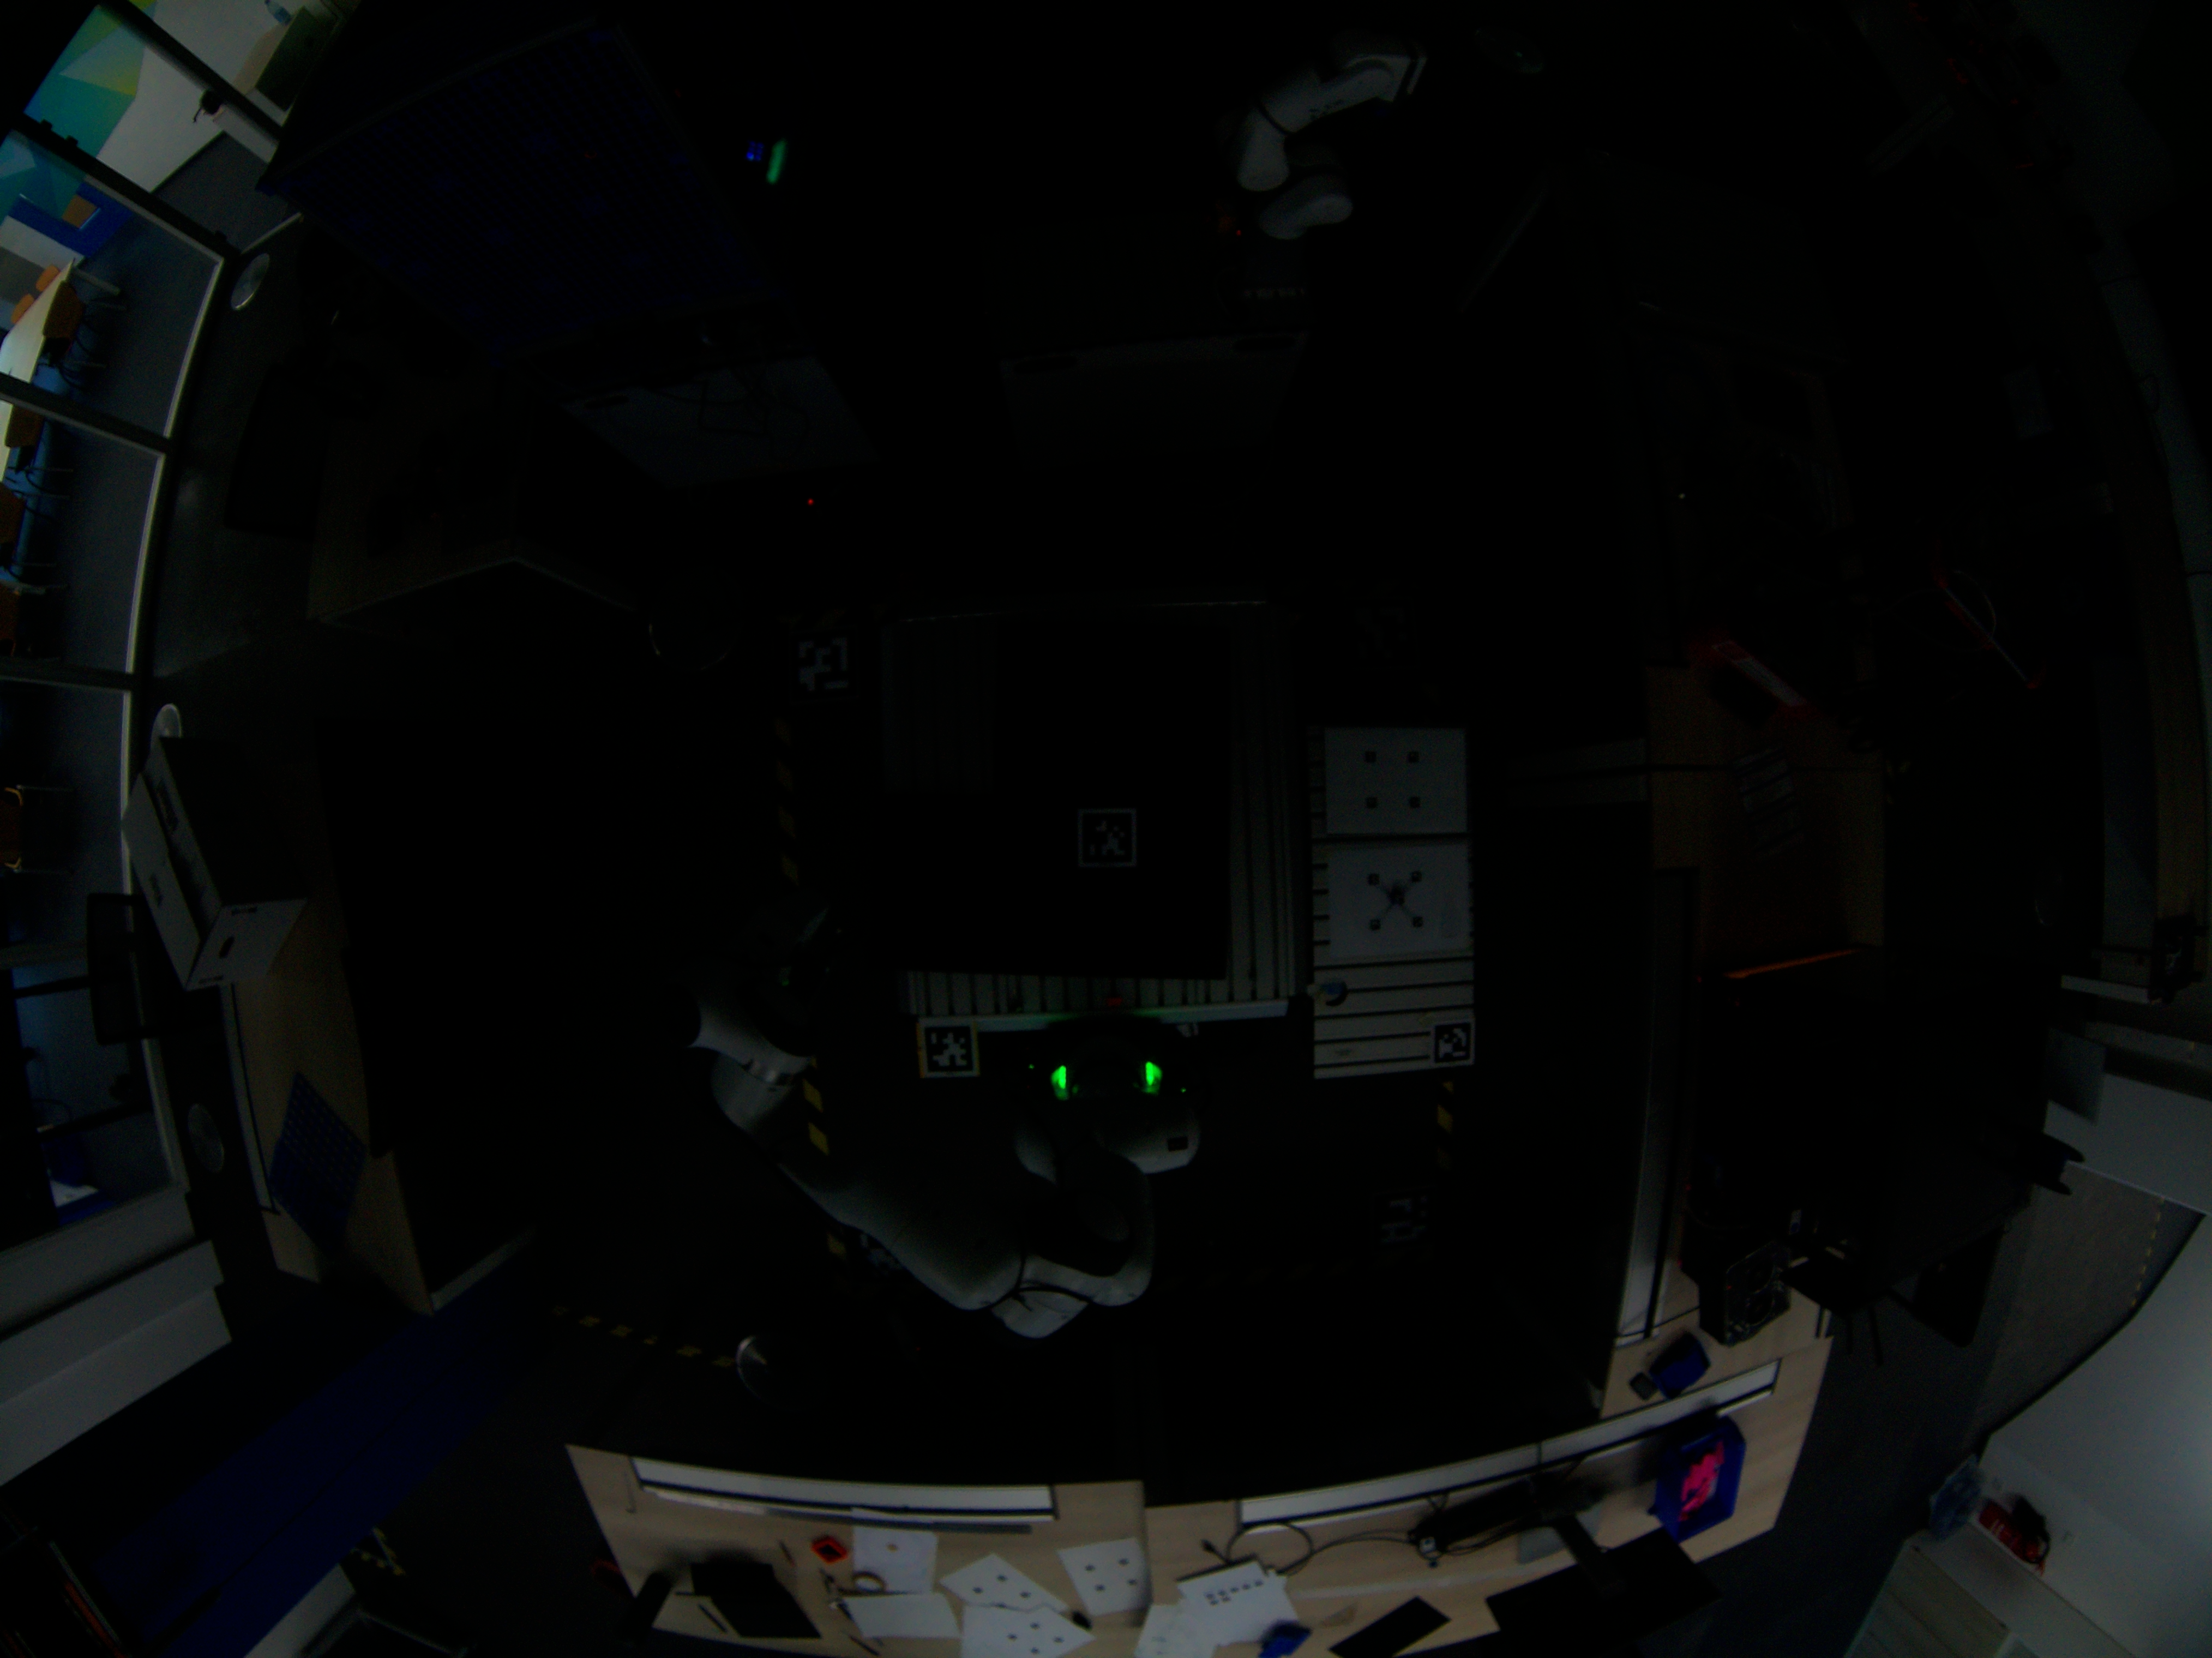
\includegraphics[width=\textwidth]{Bilder/Kapt6/Decken_Kamera_Lichttest_Fix.png}
        \caption{Deckenkamera, feste Belichtung}
        \label{fig:Decke_Lichttest_Fix}
    \end{subfigure}
    \hspace{0.8cm}
    \begin{subfigure}[t]{0.35\textwidth}
        \centering
        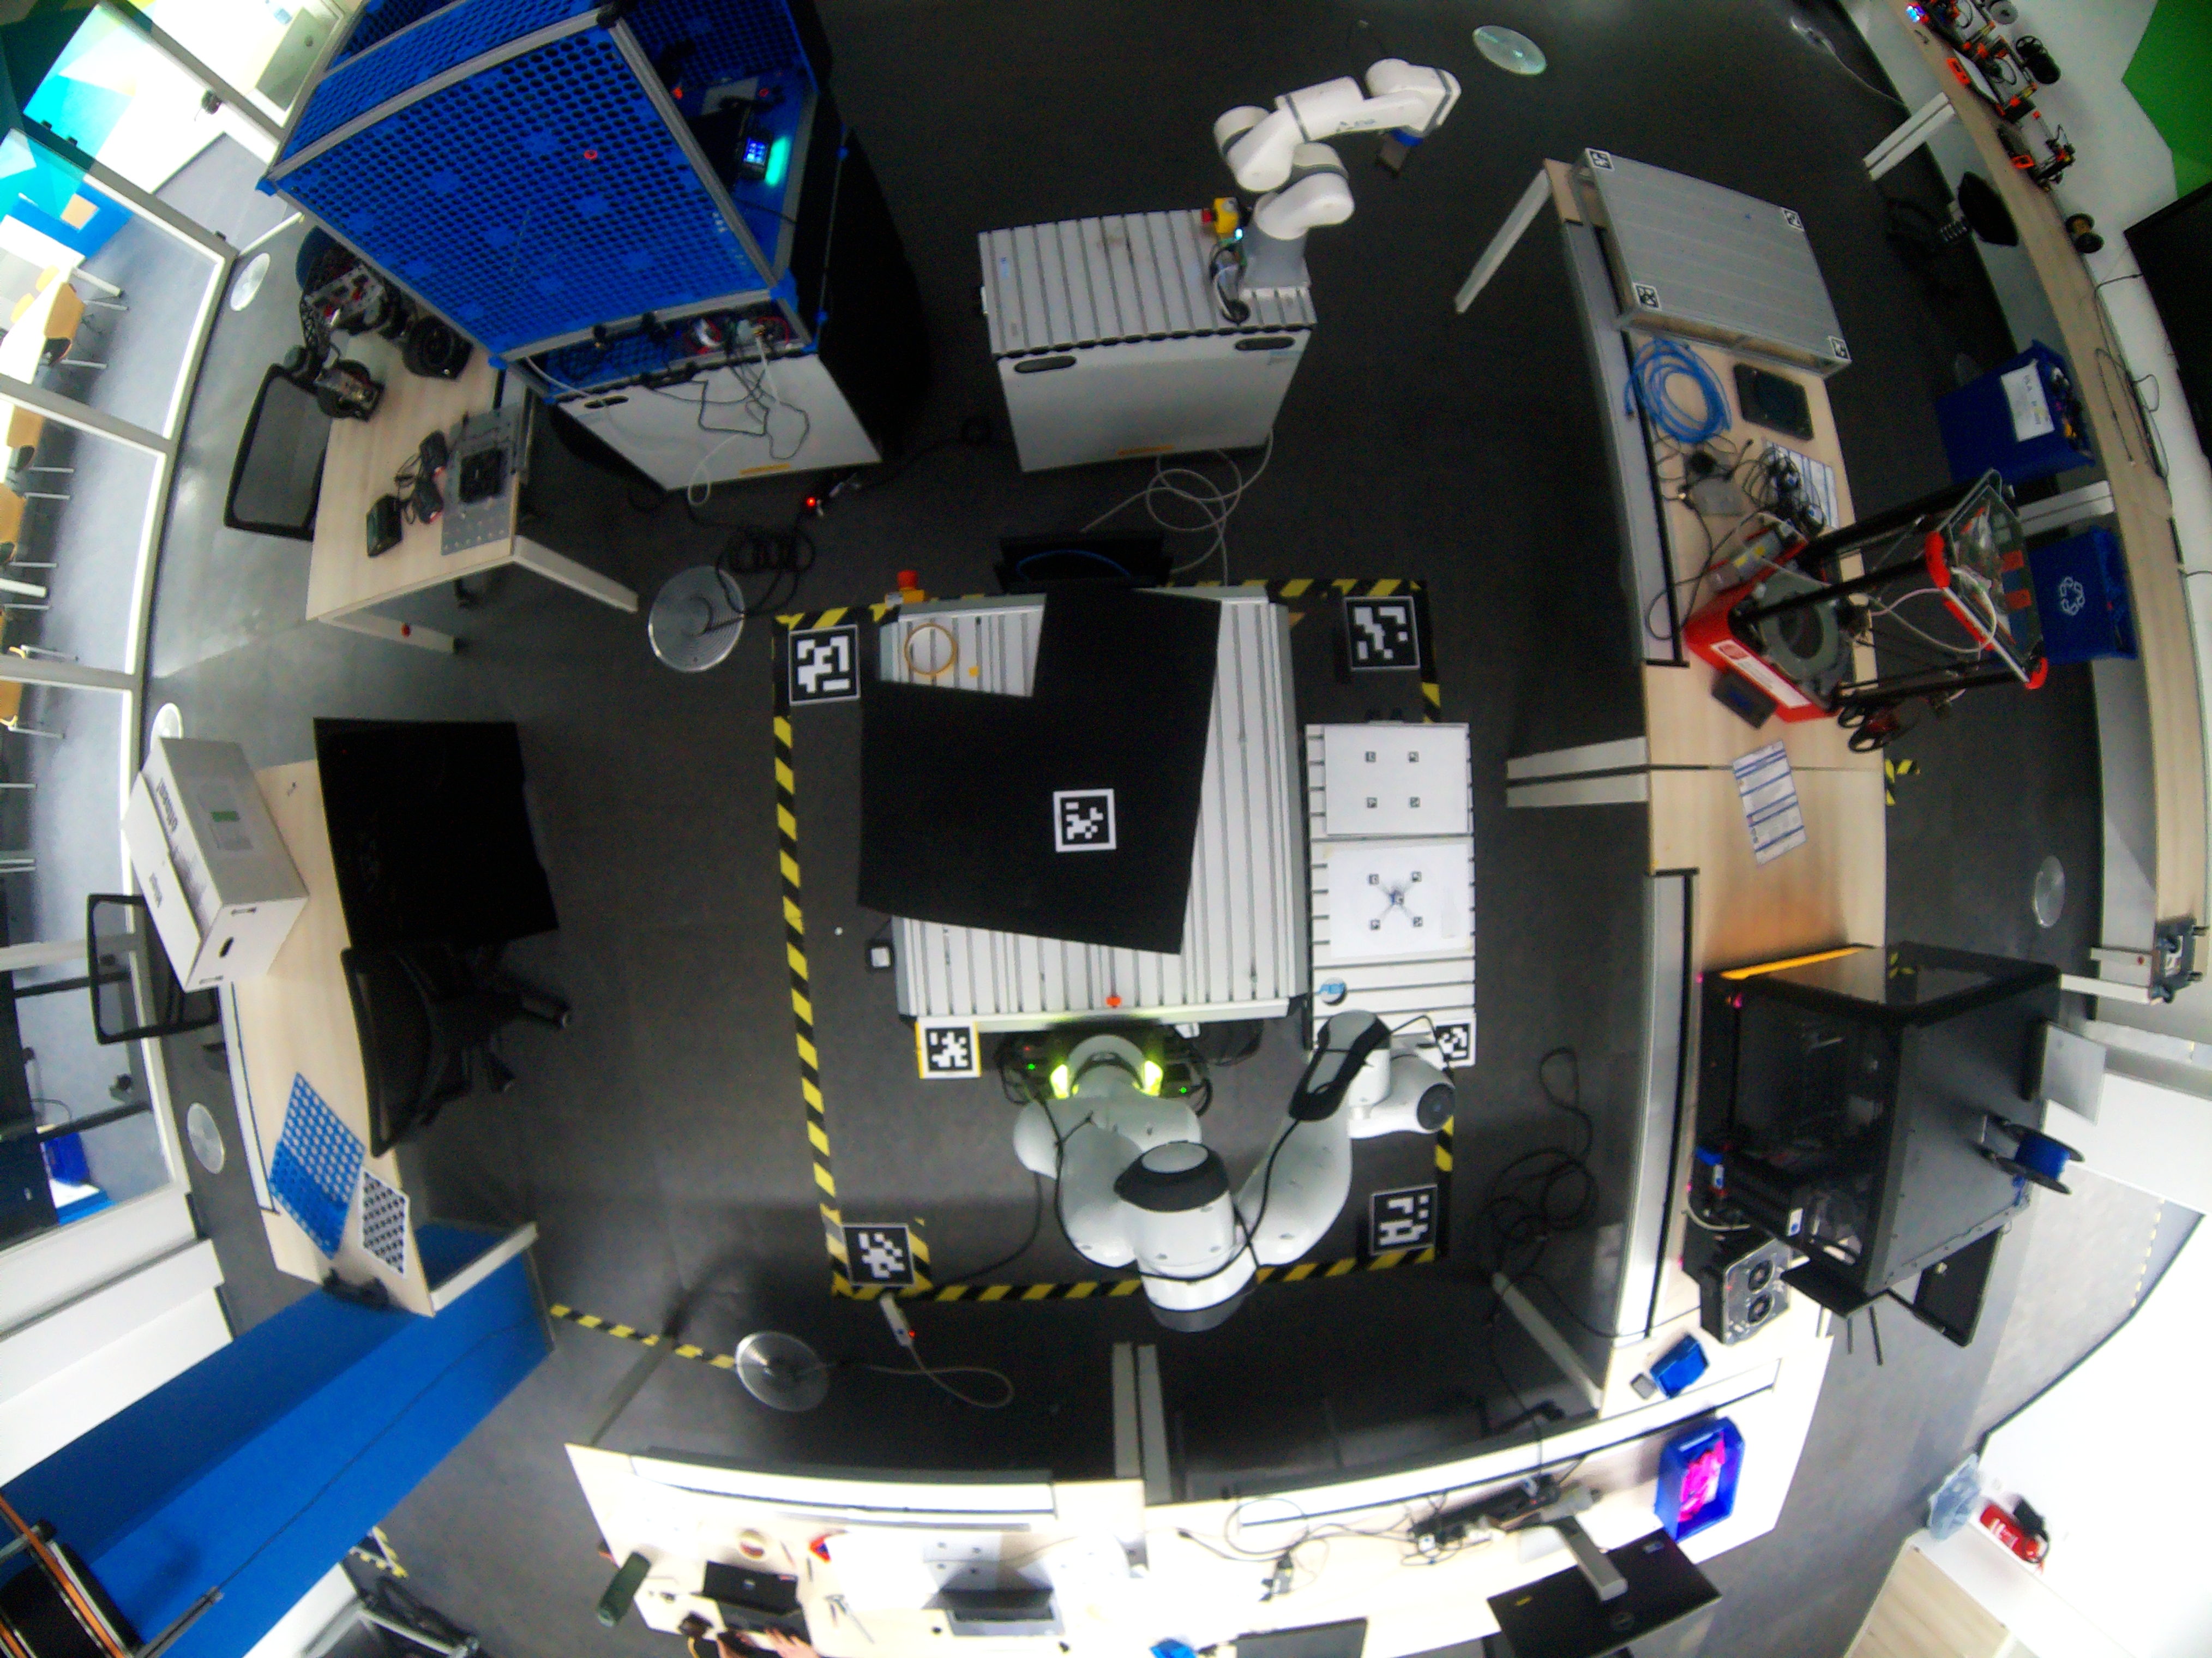
\includegraphics[width=\textwidth]{Bilder/Kapt6/Decken_Kamera_Lichttest_Auto.png}
        \caption{Deckenkamera, automatische Belichtung}
        \label{fig:Decke_Lichttest_Auto}
    \end{subfigure}

    \vspace{0.4cm}

    \begin{subfigure}[t]{0.35\textwidth}
        \centering
        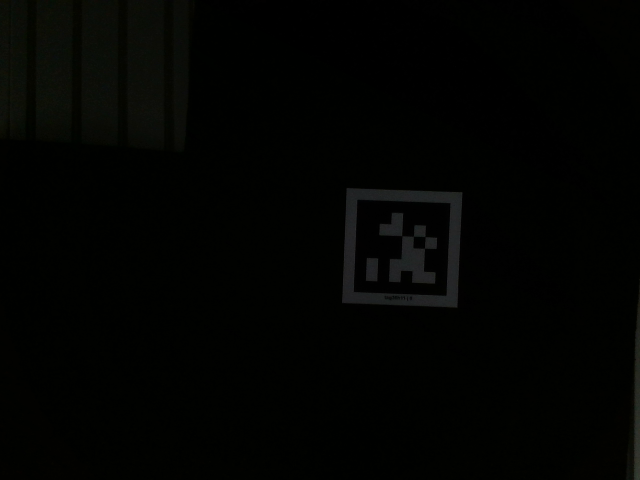
\includegraphics[width=\textwidth]{Bilder/Kapt6/Hand_Kamera_Lichttest_Fix.png}
        \caption{Handkamera, feste Belichtung}
        \label{fig:Hand_Lichttest_Fix}
    \end{subfigure}
    \hspace{0.8cm}
    \begin{subfigure}[t]{0.35\textwidth}
        \centering
        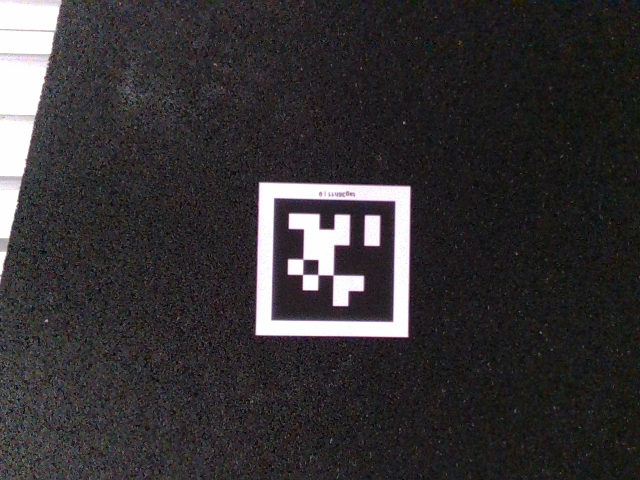
\includegraphics[width=\textwidth]{Bilder/Kapt6/Hand_Kamera_Lichttest_Auto.png}
        \caption{Handkamera, automatische Belichtung}
        \label{fig:Hand_Lichttest_Auto}
    \end{subfigure}

    \caption{Aufnahmen bei 0\,\% Beleuchtung mit fester Belichtung (Einstellung bei 100\,\% Beleuchtung) und mit automatischer Belichtung}
    \label{fig:lichttest_belichtung}
\end{figure}

Zur Beschreibung der Bildqualität wird zusätzlich der Michelson-Kontrast zwischen den weißen und schwarzen Bereichen des Tags bestimmt:
\begin{equation}
    C_M = \frac{I_{\max} - I_{\min}}{I_{\max} + I_{\min}}
    \label{eq:michelson}
\end{equation}
Dabei bezeichnet $C_M$ den Michelson-Kontrast, $I_{\max}$ den mittleren Grauwert der weißen und $I_{\min}$ den mittleren Grauwert der schwarzen Bereiche des Tags. Der Kontrast liegt zwischen 0 und 1, wobei 0 keinem und 1 dem maximal möglichen Kontrast entspricht. Abbildung~\ref{fig:Tags_Lichttest} zeigt die Aufnahmen beider Kameras bei voller und ausgeschalteter Beleuchtung.

\begin{figure}[H]
    \centering
    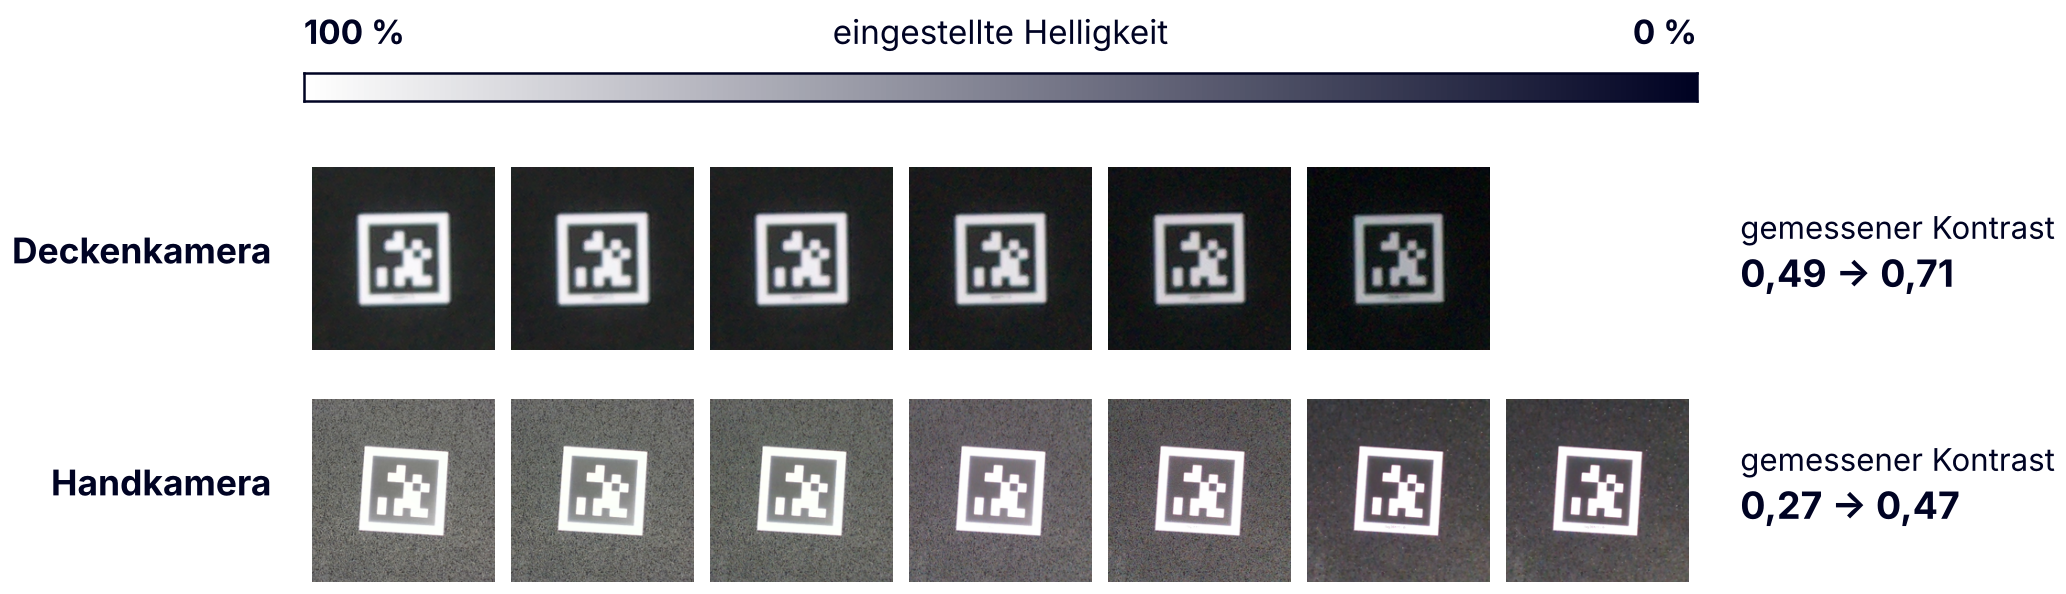
\includegraphics[width=0.9\textwidth]{Bilder/Kapt6/helligkeit_kompakt_kontrast.png}
    \caption{Aufnahmen des Tags durch Decken- und Handkamera bei 100\,\% und 0\,\% Beleuchtung mit dem jeweils gemessenen Michelson-Kontrast}
    \label{fig:Tags_Lichttest}
\end{figure}

Wie Abbildung~\ref{fig:Licht_test_kontrast} zeigt, steigt der Kontrast mit abnehmender Beleuchtung an. Physikalisch sinkt die Leuchtdichte der weißen und schwarzen Bereiche proportional zur Beleuchtung, sodass der Kontrast des gedruckten Tags konstant bleibt. Die Veränderung entsteht daher durch die nichtlineare Bildverarbeitung der Kameras. Die Grauwerte sind auf den Bereich von 0 bis 255 begrenzt. Bei der Handkamera liegen die weißen Bereiche bereits bei voller Beleuchtung im Sättigungsbereich, obwohl sie physikalisch kein reines Weiß darstellen. Sinkt die Beleuchtung, bleibt ihr Grauwert daher nahezu unverändert, während die schwarzen Bereiche deutlich dunkler abgebildet werden. Bei der Handkamera sinkt der Grauwert der weißen Bereiche zwischen voller und ausgeschalteter Beleuchtung lediglich um 0,1\,\%, der der schwarzen Bereiche hingegen um 37,5\,\%. Bei der Deckenkamera sinken die Grauwerte um 28,2\,\% beziehungsweise 63,7\,\%. Da die schwarzen Bereiche in beiden Fällen überproportional abnehmen, steigt der Kontrast.

\begin{figure}[htbp]
    \centering
    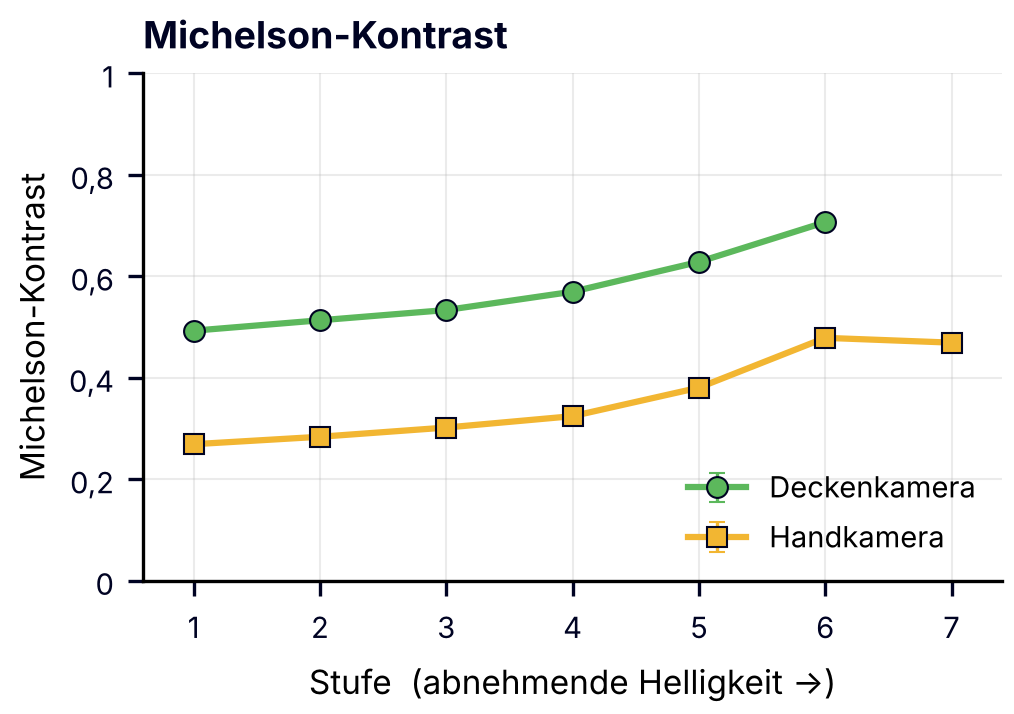
\includegraphics[width=0.5\textwidth]{Bilder/Kapt6/plot_michelson_stufen.png}
    \caption{Michelson-Kontrast des Tags über die Beleuchtungsstufen}
    \label{fig:Licht_test_kontrast}
\end{figure}

Ein höherer Kontrast führt jedoch nicht zu einer messbaren Verbesserung der Erkennung, da diese bereits bei voller Beleuchtung vollständig gelingt. Wie Abbildung~\ref{fig:Licht_test_erkennungsrate} zeigt, wird der Tag in jeder Beleuchtungsstufe ohne Bitfehler erkannt (siehe \ref{fig:Licht_test_erkennungsrate}). Die Auswertung mit \textit{pupil-apriltags} liefert identische Ergebnisse und ist zur besseren Übersicht nicht zusätzlich dargestellt.

\begin{figure}[htbp]
    \centering
    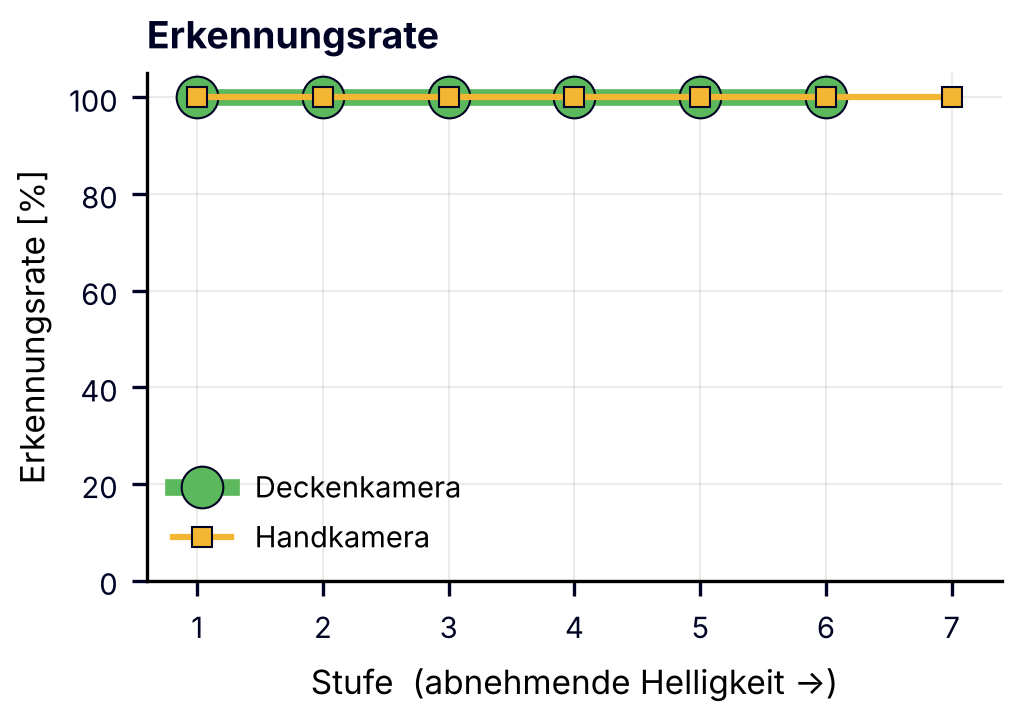
\includegraphics[width=0.5\textwidth]{Bilder/Kapt6/plot_erkennungsrate_stufen.png}
    \caption{Erkennungsrate des Tags über die Beleuchtungsstufen (Auswertung mit OpenCV)}
    \label{fig:Licht_test_erkennungsrate}
\end{figure}

Die geringere Lichtmenge gleichen die Kameras durch eine höhere Verstärkung (\textit{Gain}) aus, die das Bildrauschen ebenfalls verstärkt. Dies wirkt sich auf die Stabilität der Positionsbestimmung aus (Abbildung~\ref{fig:Licht_test_positionsbestimmung}). Bei der Handkamera steigt die mittlere Verschiebung der erkannten Tagposition zwischen den Aufnahmen mit abnehmender Beleuchtung von 0,02\,mm auf 0,05\,mm, bei der Deckenkamera von 0,25\,mm auf knapp 1\,mm. Da sich der Tag zwischen den Aufnahmen nicht bewegt, sind diese Verschiebungen ausschließlich auf das Bildrauschen zurückzuführen. Die Deckenkamera weist dabei auf allen Beleuchtungsstufen ein deutlich stärkeres Rauschen der Positionsbestimmung auf als die Handkamera.

\begin{figure}[htbp]
    \centering
    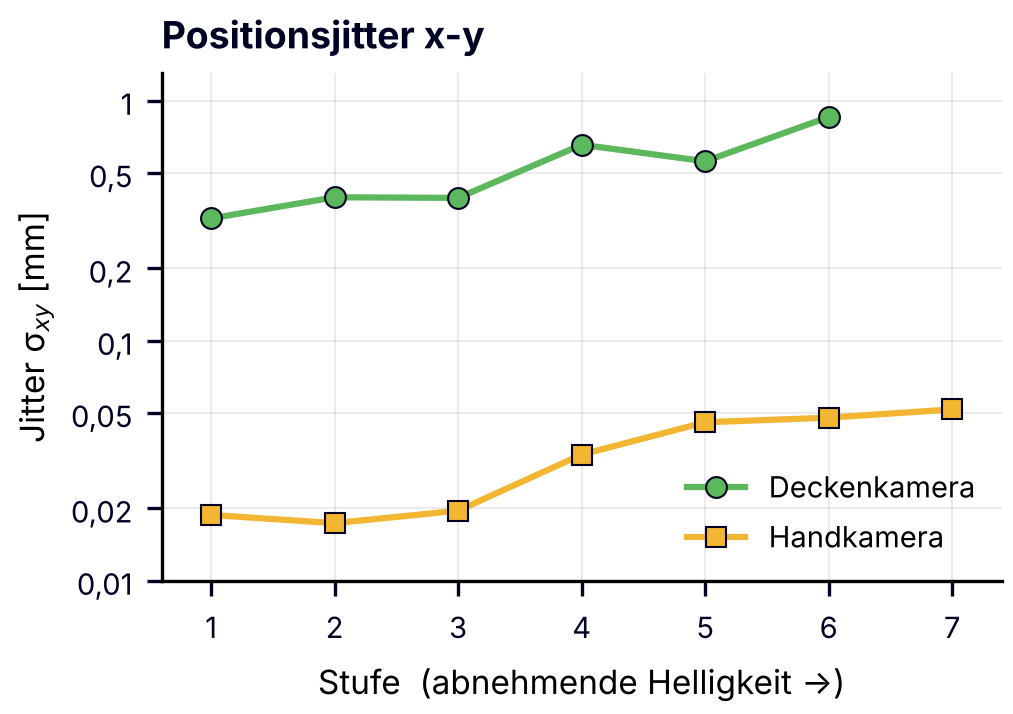
\includegraphics[width=0.5\textwidth]{Bilder/Kapt6/plot_jitter_xy_stufen.png}
    \caption{Mittlere Verschiebung der erkannten Tagposition in der $x$-$y$-Ebene innerhalb der 25 Aufnahmen je Beleuchtungsstufe}
    \label{fig:Licht_test_positionsbestimmung}
\end{figure}

Die Identifikation der Module ist somit über den gesamten untersuchten Beleuchtungsbereich zuverlässig möglich.

% =====================================================================
\subsection{Einfluss von Verdeckungen}
% =====================================================================

Der Einfluss von Verdeckungen wird simulativ untersucht. Dazu werden je ein Bild der Decken- und der Handkamera in ihrer tatsächlichen Auflösung gezielt teilweise verdeckt und mit derselben Konfiguration ausgewertet, die im realen System implementiert ist. Simuliert werden Verdeckungen an unterschiedlichen Positionen des Tags mit schwarzen und weißen Verdeckungsobjekten (Abbildung~\ref{fig:verdeckungs_test}). Tabelle~\ref{tab:verdeckung} fasst den Verdeckungsgrad zusammen, ab dem die Erkennung ausfällt.

Dabei sind zwei Mechanismen zu unterscheiden: Ob ein Tag erkannt wird, hängt von der Verdeckung des äußeren Rahmens ab. Ob seine ID korrekt ausgelesen wird, hängt von der Verdeckung der inneren Datenfelder ab.

Die Versuche E1a bis E2 untersuchen die Verdeckung des Rahmens. Sie zeigen, dass insbesondere weiße Verdeckungen in der Mitte einer Kante die Erkennung unmittelbar verhindern: Bereits eine Verdeckung von 0,5\,\% der Kantenlänge führt zum Ausfall. Weiße Verdeckungen unterbrechen den dunklen Rahmen und stellen damit die kritischste der untersuchten Verdeckungsarten dar. Schwarze Verdeckungen sind hingegen deutlich unkritischer, da sie mit dem schwarzen Rahmen verschmelzen.

Die Versuche E3 bis E5 untersuchen die Verdeckung der Datenfelder. Sie zeigen, dass nicht die verdeckte Fläche entscheidend ist, sondern die Anzahl der dadurch verfälschten Datenbits. Die zulässige Anzahl korrigierbarer Bitfehler wird in OpenCV über den Parameter \texttt{errorCorrectionRate} festgelegt. Im implementierten System ist dieser auf 0,6 eingestellt. Für die Tag-Familie tag36h11 entspricht dies bis zu drei korrigierbaren Bitfehlern, ab dem vierten Bitfehler wird die Erkennung verworfen. % TODO: In Tabelle E5 versagt die Deckenkamera bereits bei 3 Bits. Prüfen!
In keinem der simulierten Versuche wird eine falsche ID ausgegeben. Bei zu vielen Bitfehlern wird die Erkennung stattdessen verworfen, was dem gewünschten Verhalten entspricht.

Wird ein Tag nicht erkannt, werden weder eine Position noch eine ID ausgegeben. Kritisch ist jedoch eine schwarze Verdeckung entlang einer Außenkante, die mit dem Rahmen verschmilzt. Der Tag wird dann zwar erkannt, erscheint aber größer, als er tatsächlich ist. Da die Entfernung zur Kamera aus der abgebildeten Taggröße berechnet wird, verfälscht dies vor allem die Position entlang der optischen Achse, die $z$-Komponente. Diese ist ohnehin die am ungenauesten bestimmte Komponente (vgl. Abschnitt~[TODO]) und wird für die Positionierung nicht verwendet. Die Identifikation des Moduls ist davon nicht betroffen.

\begin{table}[htbp]
    \centering
    \caption{Verdeckungsgrad, ab dem die Erkennung ausfällt, für verschiedene Verdeckungsarten}
    \label{tab:verdeckung}
    \small
    \renewcommand{\arraystretch}{1.2}
    \begin{tabular}{>{\raggedright\arraybackslash}p{5.4cm} l c c}
        \toprule
        \textbf{Versuch (Bezugsgröße)} & \textbf{Farbe}
        & \textbf{Deckenkamera} & \textbf{Handkamera} \\
        \midrule
        \multirow{2}{=}{E1a -- Kante, ab Ecke (Kantenlänge)}
            & weiß    & 6,5\,\%   & 35,5\,\% \\
            & schwarz & 93,5\,\%* & 93,5\,\%* \\
        \midrule
        \multirow{2}{=}{E1b -- Kante, mittig (Kantenlänge)}
            & weiß    & 0,5\,\%   & 0,5\,\% \\
            & schwarz & 87,5\,\%* & 87\,\%* \\
        \midrule
        \multirow{2}{=}{E1c -- Zwei Kanten, L-Form (Kantenlänge)}
            & weiß    & 10,5\,\%  & 12,5\,\%* \\
            & schwarz & 93\,\%    & 92,5\,\%* \\
        \midrule
        \multirow{2}{=}{E1d -- Vier Kanten, mittig (Kantenlänge)}
            & weiß    & 0,5\,\%   & 0,5\,\% \\
            & schwarz & 84\,\%*   & 24\,\%* \\
        \midrule
        \multirow{2}{=}{E2 -- Ecke (Tag-Fläche)}
            & weiß    & 1,6\,\%   & 2,4\,\% \\
            & schwarz & 16,4\,\%  & kein Ausfall ($>25$\,\%) \\
        \midrule
        \multirow{2}{=}{E3 -- Datenfeld, Streifen (Tag-Fläche)}
            & weiß    & 2,3\,\%   & 4,5\,\% \\
            & schwarz & 13,9\,\%  & 23,3\,\% \\
        \midrule
        \multirow{2}{=}{E4 -- Zufällige Datenzellen (Datenfeld, 36 Zellen)}
            & weiß    & 11,1\,\% (4 Zellen) & 11,1\,\% (4 Zellen) \\
            & schwarz & 11,1\,\% (4 Zellen) & 11,1\,\% (4 Zellen) \\
        \midrule
        E5 -- Invertierte Bits (Datenfeld, \texttt{errorCorrectionRate} 0,6)
            & --      & 8,3\,\% (3 Bits)    & 11,1\,\% (4 Bits) \\
        \bottomrule
    \end{tabular}

    \vspace{0.2cm}
    \parbox{\textwidth}{\footnotesize
        * Das Tag fällt hier nicht sauber aus. Bei stärkerer Verdeckung wird es zeitweise wieder erkannt.}
\end{table}

\begin{figure}[H]
    \centering
    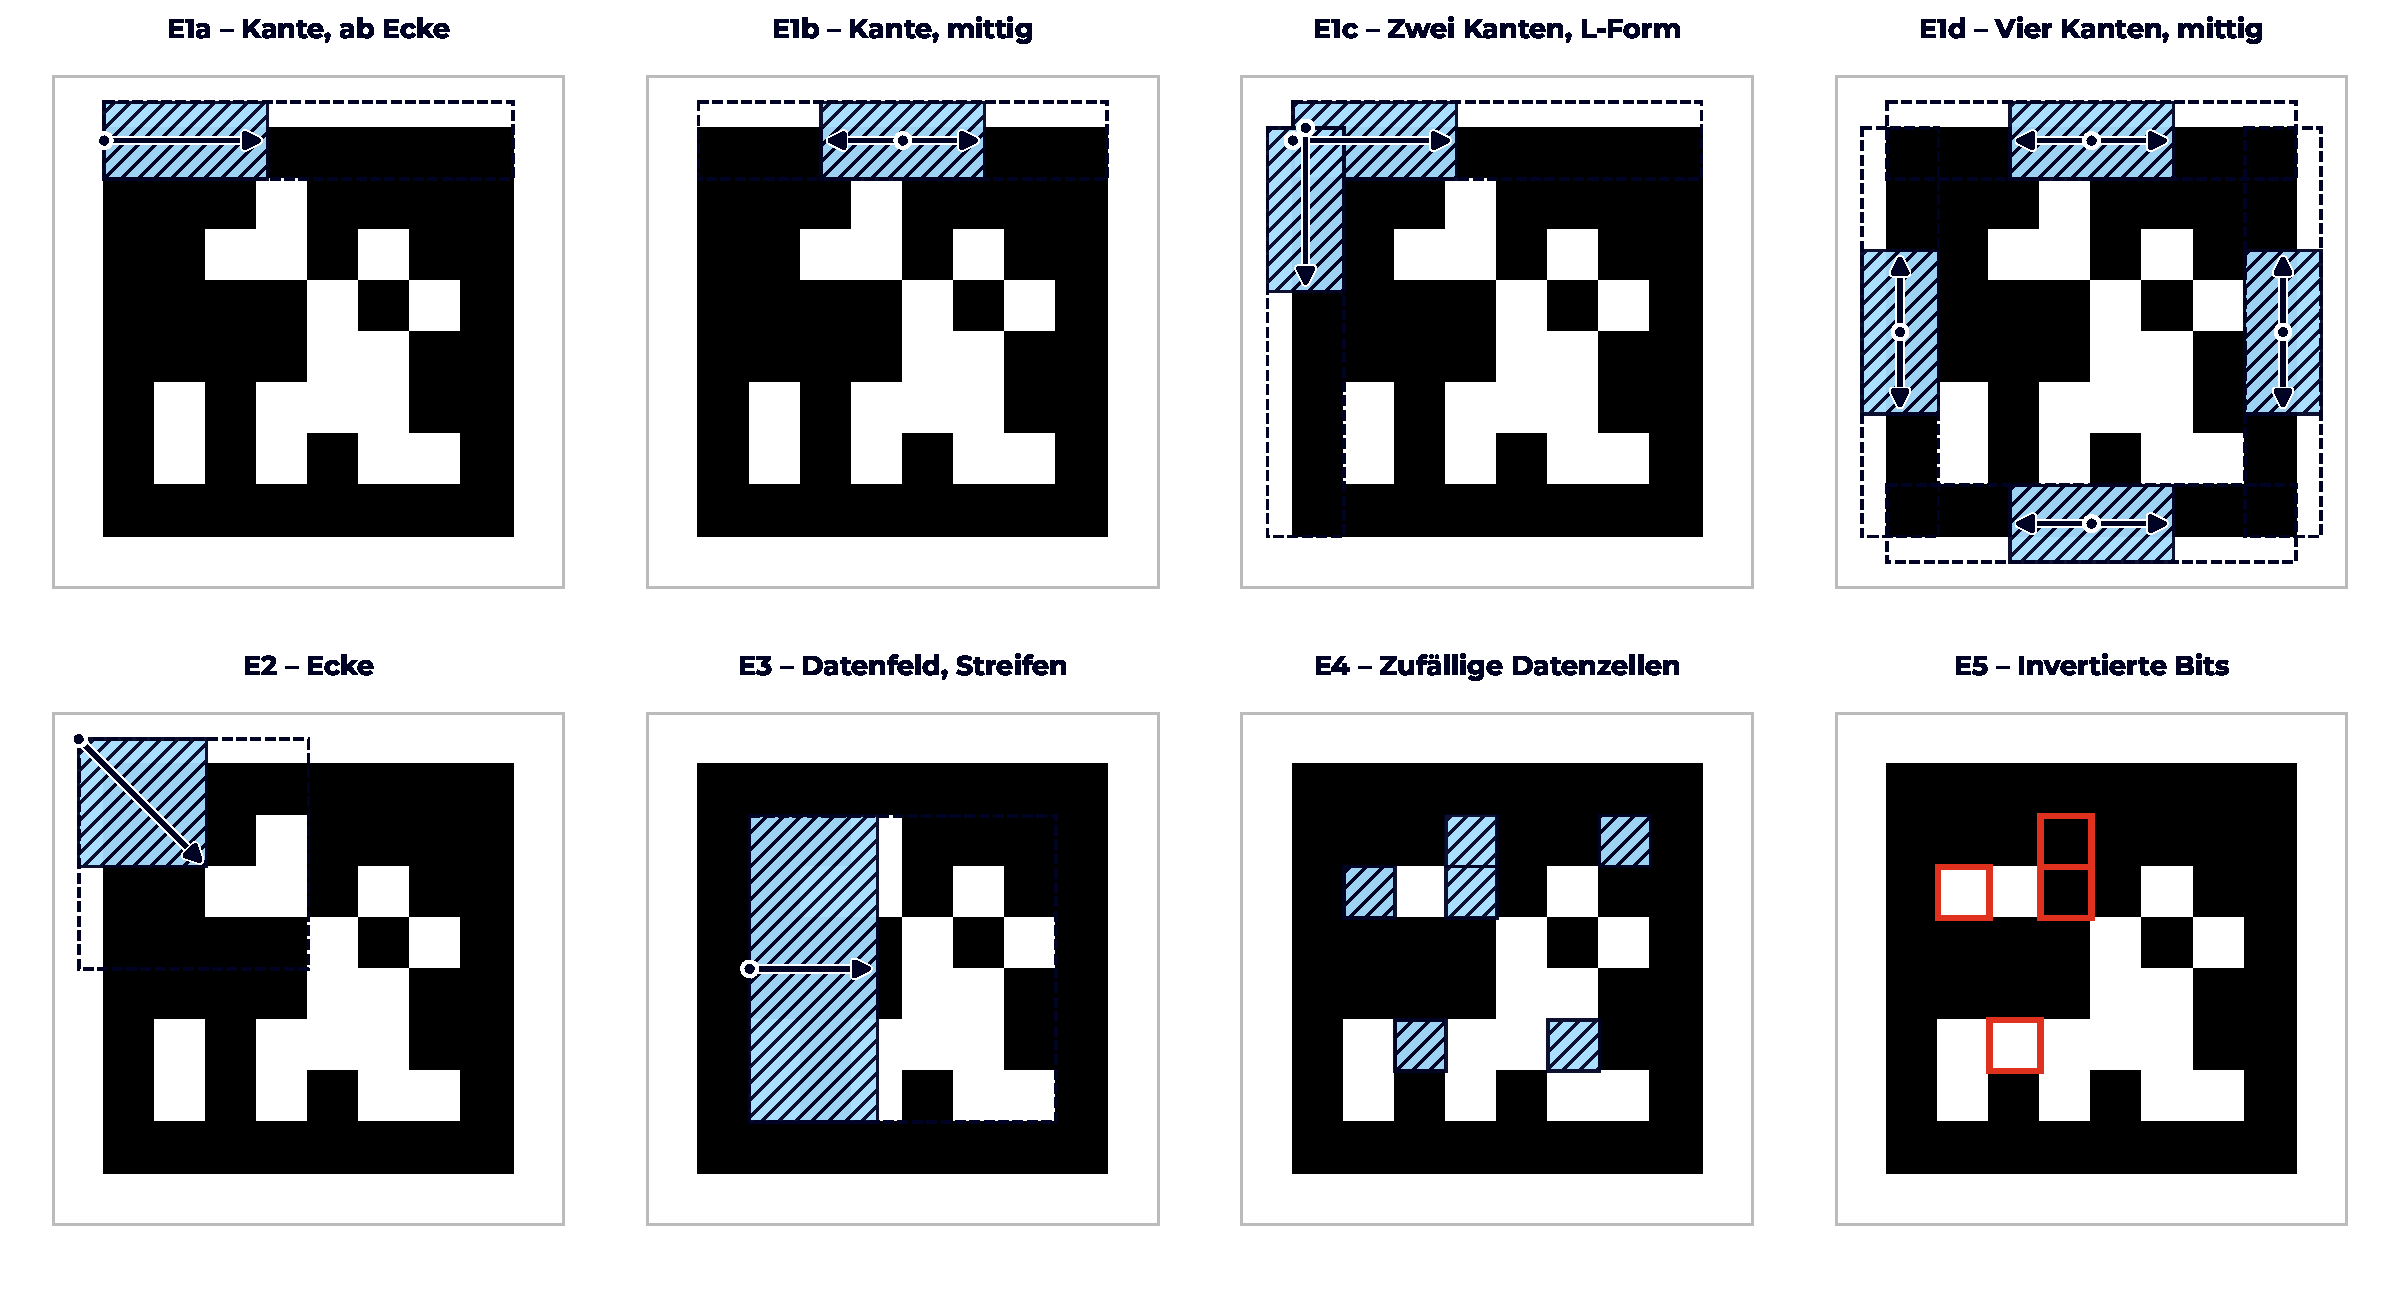
\includegraphics[width=0.9\textwidth]{Bilder/Kapt6/bericht_verdeckungstests.pdf}
    \caption{Simulierte Verdeckungsfälle der Versuche E1 bis E5}
    \label{fig:verdeckungs_test}
\end{figure}

% =====================================================================
\subsection{Bewertung}
% =====================================================================

Die Versuche zeigen, dass die Module bei allen im Arbeitsbereich auftretenden Abständen sowie über den gesamten untersuchten Beleuchtungsbereich automatisiert und zuverlässig identifiziert werden. Eine falsche ID wird in keinem der Versuche ausgegeben, sodass die Identifikation eindeutig ist. Einschränkungen ergeben sich bei Verdeckungen des Tagrahmens, insbesondere durch helle Objekte, die eine Erkennung bereits bei geringem Verdeckungsgrad verhindern. In diesem Fall wird das Modul jedoch nicht falsch, sondern gar nicht identifiziert. Der Einfluss von Verschmutzungen wurde nicht gesondert untersucht, lässt sich aber durch die simulierten Verdeckungen der Datenfelder abschätzen.

% TODO: Bewertungsstufe festlegen und an Nutzwertanalyse anpassen (siehe Hinweis im Chat).
Damit erreicht das umgesetzte System in der Anforderung \emph{Identifikation der Module} die Bewertungsstufe [TODO] und bestätigt die in der Konzeptbewertung getroffene Einschätzung.


\section{Robustheit}
\label{sec:Robustheit_Verifikation}
1 P: liefert bei Störungen unbemerkt falsche Positionen
2 P: erkennt Störungen, fällt dann aber vollständig aus
3 P: erkennt Störungen und meldet sie, Lokalisierung der nicht betroffenen
Module läuft weiter
4 P: wie 3 P, zusätzlich unempfindlich gegenüber teilweisen Verdeckungen

Lichttest + Verdeckung klären
Lv2 Wiederholgenauigkeit


\section{Kalibrierbarkeit}
\label{sec:Kalibrierbarkeit_Verifikation}
1 P: Keine Kalibrierung möglich
2 P: Kalibrierung nur mit Demontage möglich, Zeitaufwand > 8 h (eine
Person)
3 P: Kalibrierung ohne Demontage möglich, Zeitaufwand < 8 h (eine Person)
4 P: Kalibrierung ohne Demontage in < 2 h möglich (eine Person)

Wie lange dauert ein Kalibrier durchgang?
Lineal test zeigt ergebnisse vor und nach Kalibrierung

\section{Kosten}
\label{sec:Kosten_Verifikation}
1 P: 750 bis 1000 €
2 P: 500 bis 749 €
3 P: 250 bis 499 €
4 P: < 25
BOM aufzeigen

\section{Entwicklungszeit}
\label{sec:Entwicklungszeit_Verifikation}
1 P: > 12 Wochen übersteigt den zeitlichen Rahmen des ADP
2 P: < 10 --12 Wochen
3 P: < 8 --10 Wochen
4 P: < 8 Wochen

Wie lange haben wir für die Umnsetzuing gebraucht + Zeitplan

\section{Positionsgenauigkeit und Rotationsgenauigkeit}
\label{sec:Positionsgenauigkeit und Rotationsgenauigkeit_Verifikation}

% SKIZZE (28.11.2026): Methodik und Auswertekette stehen, die Unterabschnitte je Kettenglied
% enthalten nur Vorgehen und TODOs. Ergebnisse werden Schritt für Schritt ergänzt.
% Grundlage: ~/ADP/PLAN_FEHLERFORTPFLANZUNG.md, Nummern der Messungen wie in ~/ADP/messdaten/MESSUNGEN.md.

Anforderung A3 fordert eine Positioniergenauigkeit von \qty{\pm 3}{\milli\metre}. Wir werten sie so aus, dass \qty{95}{\percent} der Ablagen innerhalb eines Kreises mit \qty{3}{\milli\metre} Radius um den Sollpunkt liegen müssen. Geprüft wird das im Anwendungsfall, der Ablage eines Würfels auf einer Zielscheibe. Dieser Versuch zeigt, ob das Ziel erreicht wird. Er zeigt aber nicht, woher eine Abweichung kommt. Deshalb untersuchen wir zusätzlich die gesamte Messkette Glied für Glied.

Die Genauigkeit setzt sich aus zwei Teilen zusammen. Die Präzision beschreibt, wie stark wiederholte Messungen streuen. Die Richtigkeit beschreibt, wie weit ihr Mittelwert vom Sollwert entfernt ist. Beim Roboter entspricht das der Wiederholgenauigkeit und der Positioniergenauigkeit nach ISO~9283. % TODO Quelle ISO 9283 (nicht frei zugänglich) oder Sekundärquelle klären
Die Unsicherheiten bestimmen wir nach dem Leitfaden GUM~\cite{JCGM100}. Eine Unsicherheit vom Typ~A stammt aus eigenen Messreihen und wird als Standardabweichung angegeben. Eine Unsicherheit vom Typ~B stammt aus anderen Quellen, etwa aus einem Datenblatt. Ist dort nur eine Grenze $\pm a$ angegeben, setzen wir eine Rechteckverteilung mit $u = a/\sqrt{3}$ an.

Die Untersuchung folgt vier Schritten:
\begin{enumerate}
    \item \textbf{Messmittel:} Das Rauschen beider Kameras wird an einer ruhenden Szene bestimmt. Es ist die untere Grenze dessen, was alle weiteren Messungen auflösen können.
    \item \textbf{Glieder der Kette:} Jedes Glied wird einzeln untersucht, getrennt nach zufälligem und systematischem Anteil.
    \item \textbf{Gesamtkette:} Im Anwendungsfall wird die Abweichung der Ablage vom Ziel gemessen.
    \item \textbf{Abgleich:} Aus den Einzelbeiträgen wird eine Vorhersage für die Ablage berechnet und mit der gemessenen Abweichung verglichen.
\end{enumerate}

Für den Abgleich pflanzen wir die Einzelbeiträge durch die Kette fort. Kleine Winkelfehler lassen sich dabei linearisieren. Ein Punkt im Abstand $r$ vom Drehpunkt verschiebt sich dann um $\delta p \approx \delta t + \delta\theta \cdot r$. Diese lineare Rechnung liefert die Rangfolge der Fehlerquellen. Der radiale Fehler der Ablage ist jedoch nicht normalverteilt. Seine Verteilung und der \qty{95}{\percent}-Radius werden deshalb zusätzlich mit einer Monte-Carlo-Simulation nach~\cite{JCGM101} bestimmt. Stimmen beide Rechnungen überein, ist die Linearisierung bestätigt.

Die gemessene Abweichung der Ablage zerlegen wir in drei Ebenen. Die erste ist die Wiederholbarkeit je Pose, also die Streuung bei mehrfacher Ablage in derselben Tischlage. Die zweite ist ein Fehler, der je Tischlage fest ist, sich aber von Lage zu Lage ändert. Die dritte ist ein konstanter Versatz, der in allen Lagen gleich ist. Die erste Ebene beschreibt die Präzision, die beiden anderen die Richtigkeit.

Eine unabhängige Referenz mit höherer Genauigkeit stand nicht zur Verfügung. Die absolute Lage der Module wurde mit einem Lasermessgerät mit einer Genauigkeit von \qty{\pm 2}{\milli\metre} erfasst. Diese Messung dient nur zur Plausibilitätsprüfung. % TODO Lasermessung: Daten und Art der Genauigkeitsangabe (Grenze oder Standardabweichung) nachreichen (Meric)
Die Ablage selbst wird relativ gemessen, mit einem Kontrollfoto der Handkamera, das Zielscheibe und Würfel zugleich zeigt.

\subsection{Auswertekette}
\label{subsec:Auswertekette}

% TODO Abbildung: Messkette als Blockbild (Layer 1 grün, Layer 2 gelb), Glieder wie in Tabelle tab:auswertekette.
% TODO Klären: Gleichungen hier lassen oder in Kapitel 4 (Posenberechnung) und hier nur verweisen.

Der Ablagepunkt im Koordinatensystem der Roboterbasis ergibt sich aus der Lage der Basis und des Moduls im Weltkoordinatensystem sowie dem Ablagepunkt im Modul:
\begin{equation}
    \mathbf{p}_{B} = \left({}^{W}\mathbf{T}_{B}\right)^{-1} \, {}^{W}\mathbf{T}_{M} \, \mathbf{c}_{M}
    \label{eq:ablagepunkt}
\end{equation}
Dabei ist ${}^{A}\mathbf{T}_{B}$ die Lage von $B$ im System $A$. $W$ steht für die Welt, $B$ für die Roboterbasis, $M$ für das Modul. Der Ablagepunkt $\mathbf{c}_{M}$ stammt aus dem Modulkatalog.

Bei Layer~1 bestimmt die Deckenkamera ${}^{W}\mathbf{T}_{M}$ und ${}^{W}\mathbf{T}_{B}$ aus demselben Bild. Fehler in der Lage der Kamera wirken daher auf beide Größen ähnlich und heben sich teilweise auf. % TODO Klären: Wie genau wird die Basis in Layer 1 bestimmt (Roboter-Tags?)
Bei Layer~2 misst die Handkamera den Modul-Tag aus mehreren Ansichten. Je Ansicht gilt:
\begin{equation}
    {}^{B}\mathbf{T}_{\mathrm{Tag}} = \mathbf{F}(\mathbf{q}) \, \mathbf{X} \, {}^{C}\mathbf{T}_{\mathrm{Tag}}
    \label{eq:layer2_ansicht}
\end{equation}
Dabei ist $\mathbf{F}(\mathbf{q})$ die Vorwärtskinematik bei den Gelenkwinkeln $\mathbf{q}$, $\mathbf{X}$ das Ergebnis der Hand-Auge-Kalibrierung und ${}^{C}\mathbf{T}_{\mathrm{Tag}}$ die Lage des Tags in der Kamera. Da das Ergebnis über die Basis in die Welt und für die Ablage wieder zurück gerechnet wird, kürzt sich ${}^{W}\mathbf{T}_{B}$ in Gleichung~\eqref{eq:ablagepunkt} heraus. Die Verankerung der Basis wirkt bei Layer~2 also nicht auf die Ablage.

Tabelle~\ref{tab:auswertekette} ordnet jedem Glied der Kette den Versuch zu, mit dem es untersucht wird. Die Unterabschnitte folgen dieser Reihenfolge.

\begin{table}[htbp]
    \centering
    \caption{Glieder der Messkette und zugehörige Versuche}
    \label{tab:auswertekette}
    \begin{tabularx}{\textwidth}{@{}l c X l@{}}
        \toprule
        Glied & Layer & Versuch & Anteil \\
        \midrule
        Messrauschen Deckenkamera & 1 & ruhende Szene, 25 Bilder & zufällig \\
        Messrauschen Handkamera & 2 & ruhende Szene je WorldTag, je 30 Bilder & zufällig \\
        Intrinsik Deckenkamera & 1 & Linealtest & systematisch \\
        Intrinsik Handkamera & 2 & Distanzstück- und Seitentest & systematisch \\
        Hand-Auge-Kalibrierung & 2 & Kalibrierläufe, Höhentest, Drehtest & beide \\
        Roboter & 2 & Wiederholgenauigkeit, Rückkehr, Kinematiktest & beide \\
        Lokalisierung der Module & 1, 2 & wiederholte Scans im Anwendungsfall, Lasermessung & beide \\
        Katalog, Greifen, Prüfmessung & 1, 2 & Nachmessung, Anwendungsfall & beide \\
        Gesamtkette & 1, 2 & Anwendungsfall (Reihe 11, Vergleich Reihe 10) & gesamt \\
        \bottomrule
    \end{tabularx}
\end{table}

\subsection{Messrauschen der Deckenkamera}
\label{subsec:Messrauschen_Decke}

Das Messrauschen beschreibt die Streuung wiederholter Messungen an einer unveränderten Szene. Es ist der zufällige Anteil des Messfehlers und begrenzt die Präzision jeder Einzelmessung. Zur Bestimmung wird eine ruhende Szene mehrfach aufgenommen und jede Aufnahme einzeln ausgewertet. Kennwert ist die Standardabweichung der berechneten Tagposition über alle Aufnahmen. Die Auswertung nutzt dieselbe Tagerkennung und Posenberechnung wie das System im Betrieb.

Die Position eines Tags wird nicht in allen Richtungen gleich genau bestimmt. Quer zur Blickrichtung ergibt sie sich unmittelbar aus der Lage des Tags im Bild. Der Abstand zur Kamera folgt dagegen aus der abgebildeten Größe des Tags. Er reagiert daher empfindlich auf Abweichungen der erkannten Ecken. Die Streuung wird deshalb in zwei Anteile zerlegt: entlang der Blickrichtung, also der Verbindungslinie zwischen Kamera und Tag, und quer dazu.

Im Versuch nahm die Deckenkamera bei unveränderter Szene und gleichbleibenden Kameraeinstellungen 25 Bilder in voller Auflösung auf, im Abstand von je fünf Sekunden. Im Bildfeld lagen zwei ModulTags mit \qty{80}{\milli\metre} und vier WorldTags mit \qty{200}{\milli\metre} Kantenlänge. Ihr Abstand zur Kamera betrug \qtyrange{1,7}{3,0}{\metre}. Abbildung~\ref{fig:positionsrauschen_decke} zeigt für jeden Tag die Abweichungen der einzelnen Messungen vom Mittelwert.

\begin{figure}[htbp]
    \centering
    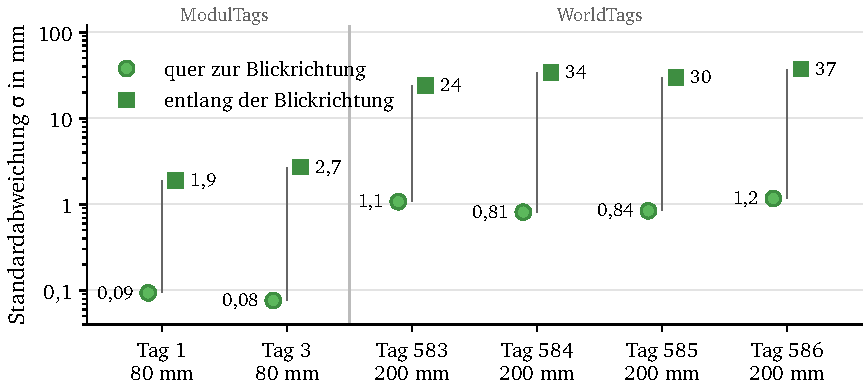
\includegraphics{Bilder/Kapt6/positionsrauschen_decke.pdf}
    \caption{Abweichung der gemessenen Tagposition vom Mittelwert je Tag aus 25 Aufnahmen einer ruhenden Szene der Deckenkamera, mit 2$\sigma$-Ellipse und projizierter Blickrichtung. Darunter die Standardabweichung quer zur und entlang der Blickrichtung.}
    \label{fig:positionsrauschen_decke}
\end{figure}

Die Messpunkte liegen bei allen Tags auf einer schmalen Ellipse. Ihre lange Achse fällt nahezu mit der projizierten Blickrichtung zusammen. Die Streuung entsteht also fast vollständig entlang der Blickrichtung. Bei den ModulTags beträgt die Standardabweichung quer zur Blickrichtung weniger als \qty{0,1}{\milli\metre} und entlang der Blickrichtung \qtyrange{1,9}{2,7}{\milli\metre}. Die WorldTags streuen in beiden Richtungen etwa um eine Größenordnung stärker, mit rund \qty{1}{\milli\metre} quer und \qtyrange{24}{37}{\milli\metre} entlang der Blickrichtung. Ursache ist die Bestimmung der Ecken auf Bruchteile eines Pixels. Bei den ModulTags arbeitet sie zuverlässig. Bei den WorldTags bleibt sie in der Mehrzahl der Aufnahmen wirkungslos, sodass die Ecken nur pixelgenau erfasst werden.

Quer zur Blickrichtung ist das Messrauschen gegenüber der geforderten Positioniergenauigkeit von \qty{\pm 3}{\milli\metre} vernachlässigbar. Entlang der Blickrichtung erreicht es dagegen eine relevante Größe, insbesondere bei den WorldTags. Über diese bestimmt die Deckenkamera ihre eigene Lage im Raum. Dieser Anteil wird daher in der Fehlerbetrachtung der Positionsgenauigkeit berücksichtigt.

\subsection{Messrauschen der Handkamera}
\label{subsec:Messrauschen_Hand}

Das Messrauschen der Handkamera wird auf dieselbe Weise bestimmt wie bei der Deckenkamera. Der Roboter steht still, die Handkamera nimmt einen WorldTag mehrfach auf, und jede Aufnahme wird einzeln ausgewertet. Da die Deckenkamera dieselben WorldTags sieht, lässt sich das Rauschen beider Kameras an denselben Tags vergleichen.

% TODO Daten: ~/ADP/messdaten/03_messkette/LV2_Messrauschen/lauf_004 bis lauf_008, je 30 Bilder,
%   WorldTags 583 (zweimal: lauf_004 11:32, lauf_005 15:16), 584, 585, 586, Abstand ca. 1,0 bis 1,3 m, 27.11.2026.
% TODO Auswertung wie Deckenkamera: Streuung quer und entlang der Blickrichtung, gleiche Abbildungsart, Systemdetektor.
% TODO Ergebnis und Vergleich mit Deckenkamera (gleiche Tags 583 bis 586).

\subsection{Intrinsische Kalibrierung der Kameras}
\label{subsec:Intrinsik}

Die intrinsische Kalibrierung legt fest, wie die Kamera einen Punkt im Raum auf das Bild abbildet. Ein Fehler darin wirkt vor allem als Maßstabsfehler und ist systematisch. Er zeigt sich daher nicht im Rauschen. Zur Prüfung werden Strecken mit bekannter Länge gemessen und mit dem Sollwert verglichen.

% TODO Deckenkamera: Linealtest (Messung 14, ~/ADP/messdaten/05_linealtest), Auswertung durch Sven. Gültige Messungen und Soll-Abstände klären.
% TODO Handkamera: Distanzstück- und Seitentest (Messungen 6 und 7), Maßstabsfehler mit eigener Kalibrierung gegen Werks-Intrinsik.

\subsection{Hand-Auge-Kalibrierung}
\label{subsec:HandAuge}

Die Hand-Auge-Kalibrierung $\mathbf{X}$ verbindet die Handkamera mit dem Flansch des Roboters. Ein Fehler in ihrer Drehung wirkt über den Abstand zwischen Kamera und Tag als Verschiebung. Er hängt daher von der Stellung des Roboters ab. Untersucht werden die Streuung zwischen mehreren Kalibrierläufen und die verbleibende Abweichung der aktiven Kalibrierung.

% TODO Daten: 7 Kalibrierläufe (Messung 12/13, ~/ADP/messdaten/04_handauge_kalibrierung),
%   Höhentest (Messung 8, 03_messkette/hoehentest, Lauf 6), Drehtest in drei Arbeitsabständen (Messung 9, Reihen 900/902/904, noch nicht ausgewertet).

\subsection{Roboter}
\label{subsec:Roboter_Genauigkeit}

Die Handkamera misst über die Kinematik des Roboters. Für die Ablage zählt daher nicht der volle Absolutfehler des Roboters, sondern nur der Unterschied zwischen der Stellung bei der Messung und der Stellung bei der Ablage. Untersucht werden die Wiederholgenauigkeit, die Rückkehr aus verschiedenen Stellungen und die Abweichung bei verschiedenen Gelenkstellungen.

% TODO Daten: Wiederholgenauigkeit (Messung 2), Rückkehrgenauigkeit (Messung 3), Kinematiktest (Messung 5), Datenblatt FR3 und Franzese2026Calibration.
% TODO Doppelzählung vermeiden: Kinematiktest enthält Kinematik und Hand-Auge zusammen.

\subsection{Lokalisierung der Module}
\label{subsec:Lokalisierung_Genauigkeit}

In diesem Glied wird die Lage eines Moduls aus den vorherigen Gliedern zusammengesetzt. Bei Layer~1 hat jeder Versuch im Anwendungsfall einen neuen Scan der Deckenkamera. Die Versuche je Tischlage sind damit Wiederholungen derselben Messung. Daraus ergibt sich die Streuung von Modullage und Basis sowie deren Zusammenhang. Bei Layer~2 wird die Streuung des zusammengeführten Ergebnisses aus mehreren Ansichten betrachtet. Die Lasermessung der Module dient als Plausibilitätsprüfung der absoluten Lage.

% TODO Daten: Reihe 11 (Layer-1-Scans je Pose), Reihe 10 zum Vergleich; Lasermessung (Meric reicht nach).
% TODO Kovarianz Modul/Basis bei Layer 1 berechnen.

\subsection{Katalog, Greifen und Prüfmessung}
\label{subsec:Katalog_Greifen}

Zwischen der gemessenen Lage des Tags und der Ablage liegen weitere Größen: die Lage des Tags am Modul und der Ablagepunkt aus dem Katalog, die Lage des Würfels im Greifer und das Absetzen. Hinzu kommt die Unsicherheit des Kontrollfotos selbst. Diese Größen werden aus Nachmessungen und aus dem Anwendungsfall abgeschätzt.

% TODO Werte: Katalog/Tag am Tisch <= 1 mm (Typ B), Zielscheibe ca. 1 mm, Würfel im Greifer (mit Greifer drehender Anteil),
%   Greifen/Absetzen zufällig aus Streuung je Pose, Prüfmessung (synthetisch <= 0,01 mm, real nicht geprüft).

\subsection{Gesamtkette im Anwendungsfall}
\label{subsec:Gesamtkette}

Im Anwendungsfall legt der Roboter einen Würfel auf eine Zielscheibe auf dem Modul ab. Gemessen wird die Abweichung vom Ziel in beiden Richtungen der Ebene sowie die Verdrehung. In jeder Tischlage wird je fünfmal nur mit Layer~1 und fünfmal mit Layer~2 abgelegt. So lassen sich beide Layer unter gleichen Bedingungen vergleichen. Die Ergebnisse werden in die drei Ebenen aus Wiederholbarkeit, lageabhängigem Fehler und konstantem Versatz zerlegt.

% TODO Daten: Reihe 11 (~/ADP/messdaten/02_use_case_reihen/main_use-case/reihe_011, sieben Posen inkl. Pose 1 neu und 180°-Test),
%   Versuch 41 ausklammern. Reihe 10 als Vergleich (zwischendurch evtl. Systemänderungen, klären welche).
% TODO Rotationsgenauigkeit (Verdrehung des Würfels) hier mit auswerten.

\subsection{Fehlerfortpflanzung und Abgleich}
\label{subsec:Fehlerfortpflanzung}

Die Ergebnisse der einzelnen Glieder werden in einem Unsicherheitsbudget zusammengefasst und mit Gleichung~\eqref{eq:ablagepunkt} bis zur Ablage fortgepflanzt. Die Vorhersage wird für jede Ebene mit der Messung im Anwendungsfall verglichen. Bleibt ein Anteil unerklärt, weist er auf eine Fehlerquelle hin, die in den Einzelversuchen nicht erfasst wurde.

% TODO Budgettabelle (8 bis 10 Zeilen: Größe, Typ, u, Beitrag), vollständige Tabelle im Anhang.
% TODO Abbildungen: Budget-Balken je Layer; Verteilung radialer Fehler (Monte Carlo) mit gemessenen Radien und 3-mm-Linie; Vorhersage gegen Messung je Pose.

\subsection{Bewertung}
\label{subsec:Bewertung_Genauigkeit}

% TODO Bewertung A3 nach den drei Ebenen. Arbeitshypothese (HYPOTHESE_ENDGENAUIGKEIT.md): Präzision von Layer 2 erfüllt ±3 mm,
%   Richtigkeit nicht (konstanter Versatz und lageabhängiger Kalibrierrest, systematisch). Folgerung für Ausblick: besseres Kalibrierkonzept.
% TODO Bewertungsstufe nach Punkteskala festlegen.


\section{Aufrüstbarkeit}
\label{sec:Aufrüstbarkeit_Verifikation}
1 P: Nicht aufrüstbar
2 P: Aufrüstung nur mit einem Arbeitsaufwand von > 8 h möglich (eine
Person)
3 P: Aufrüstung in 4 bis 8 h möglich (eine Person)
4 P: Aufrüstung in < 4 h möglich (eine Person

Der von der Fischauge abgedeckte bereich istz ja größer. ALso sehr leicht erweiterbar

Wie lange dauert es ein neues Modul einzubauen?
Meric: Habs gemessen, Tag ist schon ausgedruckt. CAD Modell existiert schon, Tag aufbringen, vermessen und dann im Modulkatalog eintragen hat 3min gedauert, hätte gesagt wir sagen 5min schafft das jeder





